\documentclass[aps,pra,superscriptaddress,twocolumn]{revtex4-1}

\usepackage{graphicx}
\usepackage{amsmath}
\usepackage{amssymb}
\usepackage{hyperref}
\usepackage[utf8]{inputenc}
\usepackage{mathtools}
\usepackage[english]{babel}
\usepackage{bbm}
\hypersetup{colorlinks=true, linkcolor=blue, citecolor=blue, urlcolor=blue}
\usepackage{xcolor}
\usepackage{braket}

%===Newcommands============================
\DeclareMathOperator{\sgn}{sgn}
\newcommand{\ie}{i.\,e.,\ }
\newcommand{\Ie}{I.\,e.\,,\ }
\newcommand{\eg}{e.\,g.,\ }
\newcommand{\Eg}{E.\,g.\,,\ }
\newcommand{\cf}{cf.\ }
%
\newcommand{\re}{\mathrm{Re}}
\newcommand{\im}{\mathrm{Im}}
\newcommand{\abs}[1]{|#1|}
\newcommand{\ii}{\mathrm{i}}
\newcommand{\ee}{\mathrm{e}}
\newcommand{\proj}[1]{|#1\rangle\langle #1|}
\newcommand{\Tr}{\operatorname{Tr}}
\newcommand{\rr}{\mathbf{r}}
\newcommand{\pp}{\mathbf{p}}
\newcommand{\kk}{\mathbf{k}}
%
\newcommand{\cc}{\text{c.c.}}
\newcommand{\fref}[1]{\text{Fig.}~\ref{#1}}
\newcommand{\ffref}[1]{\text{Figs.}~\ref{#1}}
\newcommand{\eref}[1]{\text{Eq.}~\eqref{#1}}
\newcommand{\eeref}[1]{\text{Eqs.}~\eqref{#1}}
%
\newcommand{\commentSB}[1]{\texttt{\color{blue}[#1]}}
\newcommand{\commentSO}[1]{\texttt{\color{orange}[#1]}}
\newcommand{\commentTP}[1]{\texttt{\color{green}[#1]}}
\newcommand{\commentOR}[1]{\texttt{\color{yellow}[#1]}}
\newcommand{\commentSY}[1]{\texttt{\color{red}[#1]}}

%==============================================================================================
\begin{document}
\title{title}
\author{A}
\email{}
\affiliation{Department of Physics, Harvard University, Cambridge, Massachusetts 02138, USA}
\author{B}
\email{}
\affiliation{Department of Physics, Harvard University, Cambridge, Massachusetts 02138, USA}
\author{C}
\email{}
\affiliation{Department of Physics, Harvard University, Cambridge, Massachusetts 02138, USA}

\begin{abstract}

This is the abstract. 

\end{abstract}

\maketitle

%==============================================================================================
\section{Introduction}

This is the introduction, see \commentSB{not sure about this statement}~\fref{fig:setup}.

\begin{equation}
H = p^2
\label{eqn:Hamiltonian}
\end{equation}

\begin{figure}
\centering
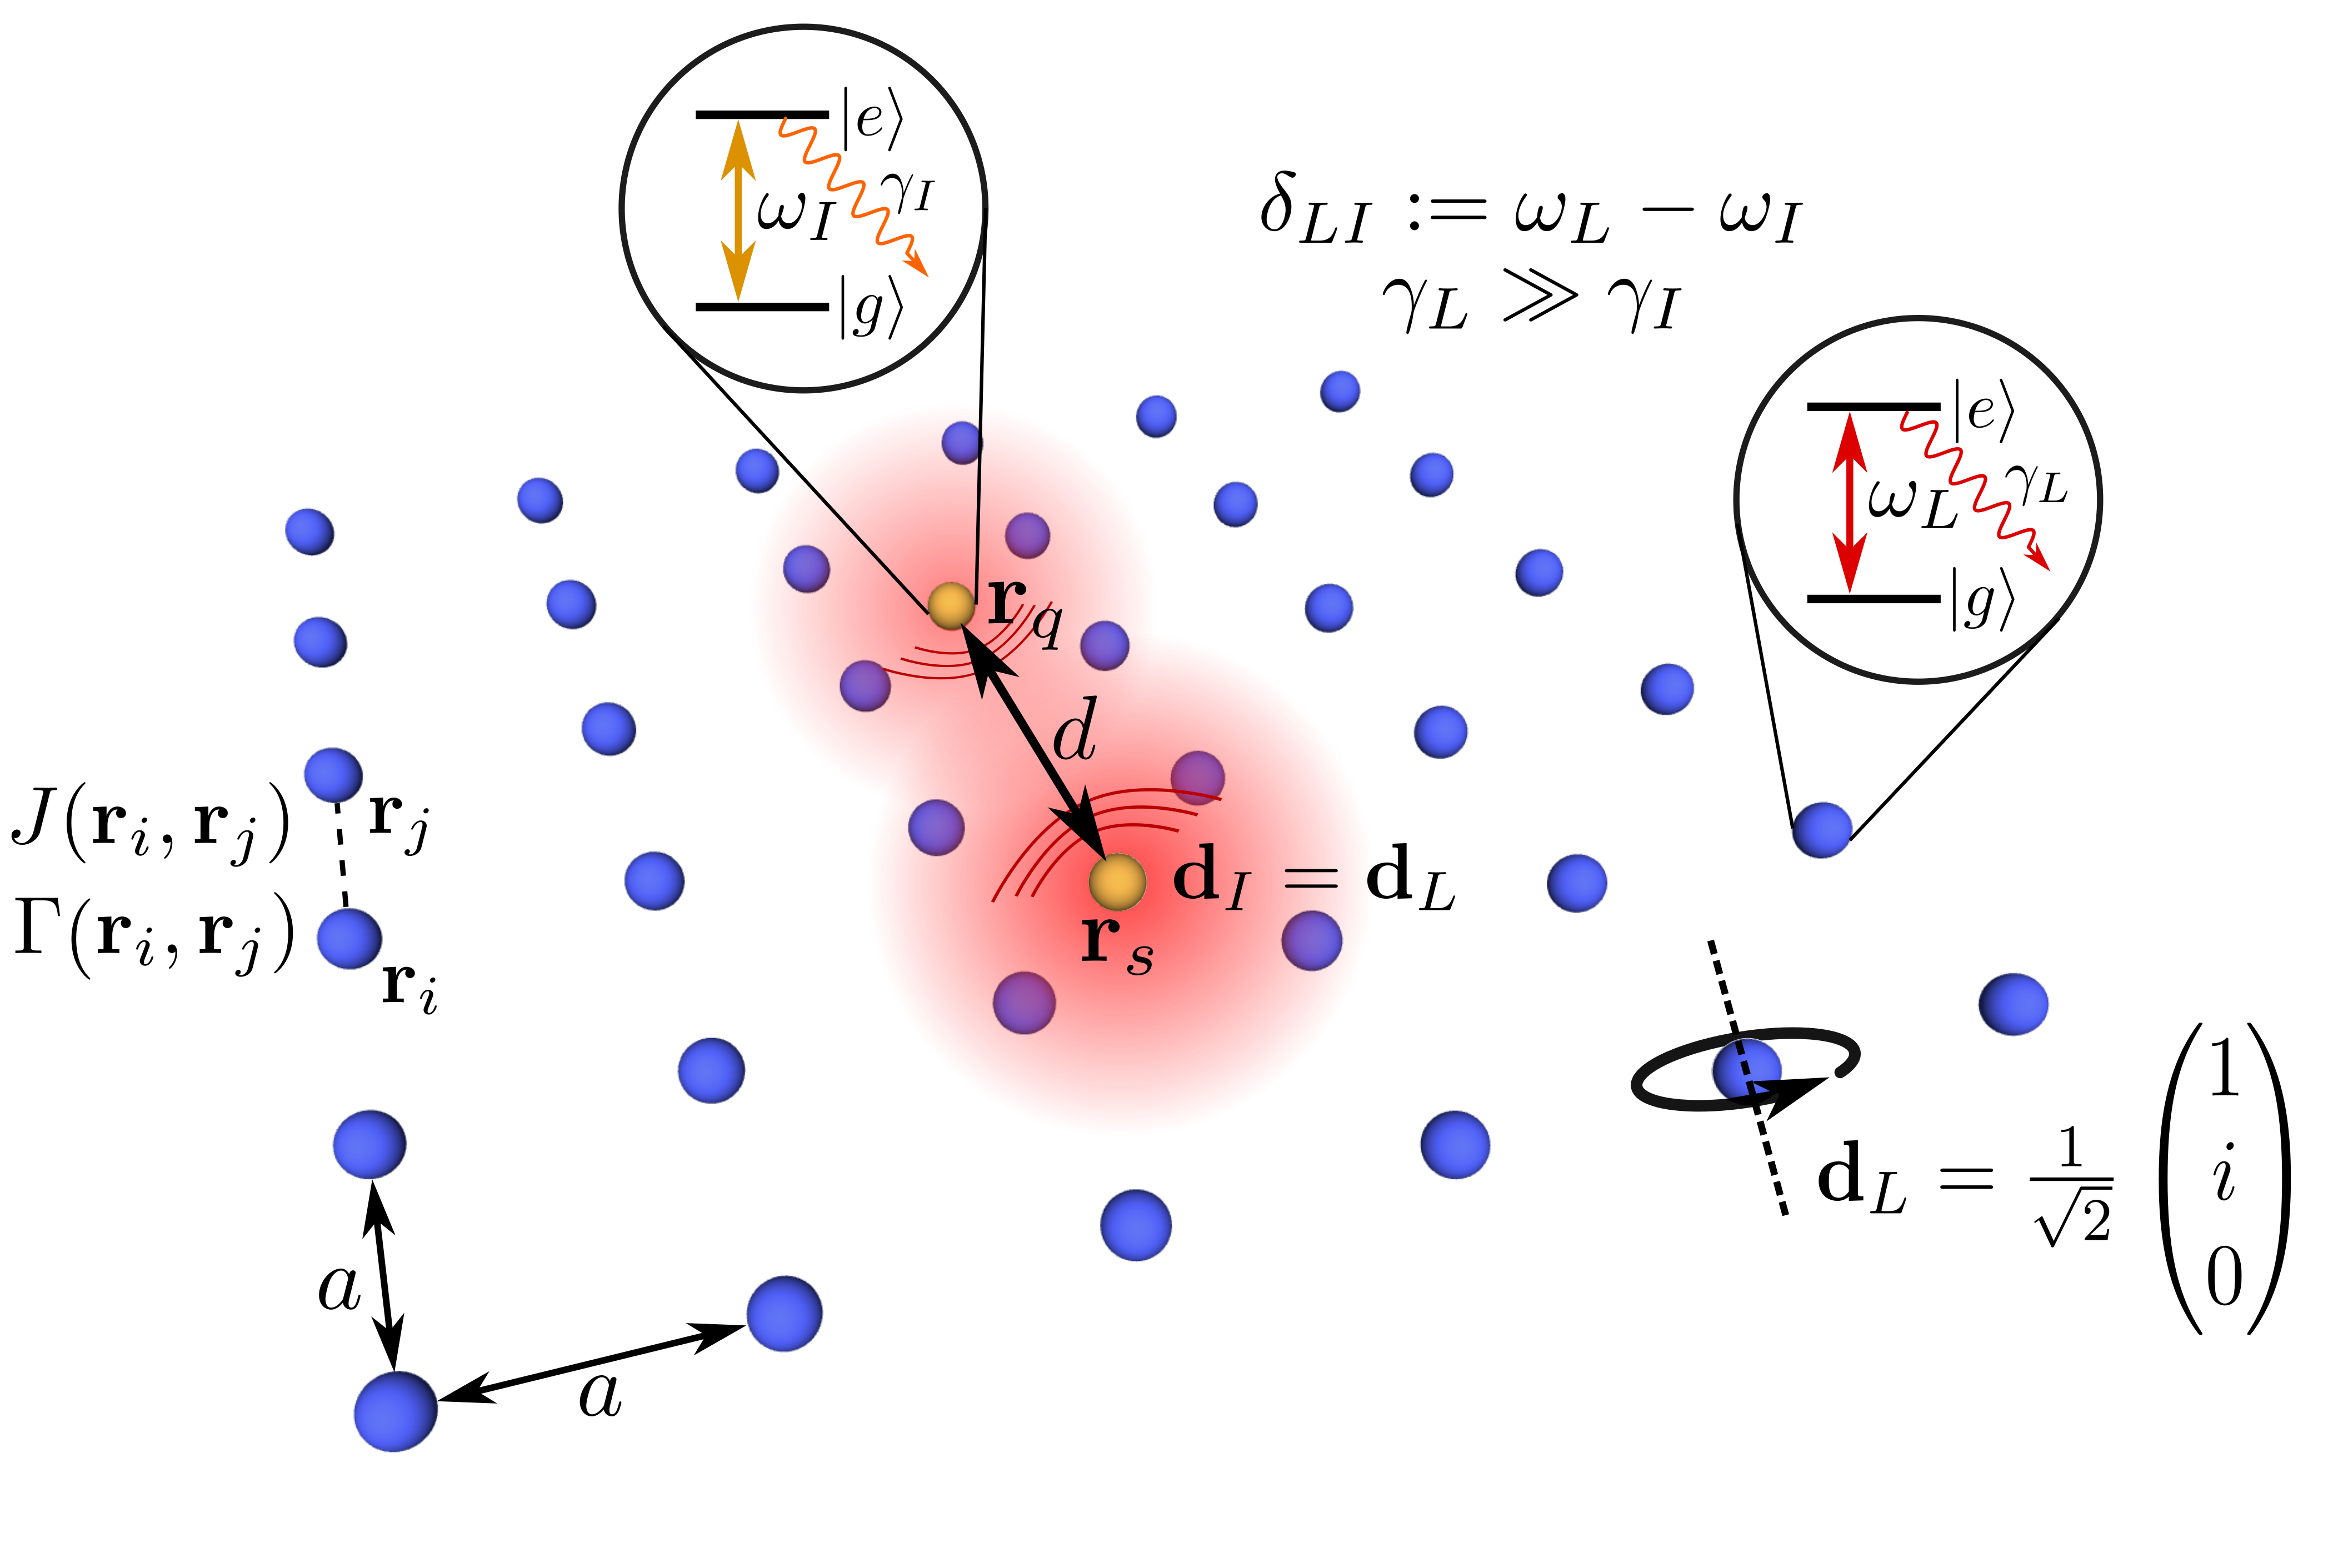
\includegraphics[width=0.4\textwidth]{figures/setup_2.png} 
\caption{•}
\label{fig:setup}
\end{figure}

We see in~\eeref{eqn:Hamiltonian} and~\fref{fig:setup},~\eg test~\cite{cidrim_photon_2020}

%==============================================================================================
\section{Model}
\commentSO{arb. geometry, Green's Tensor, Couplings, Polarizations -> Distance dependence, Hamiltonian, Self-energy, Ref. to Taylor's work}

%==============================================================================================
\section{Single impurity case}
\commentSO{Define lattices, define distances related to lattices, $\Gamma_\mathrm{eff}$, constant area}

\subsection{Square vs. triangular}

%=================
\subsubsection{Interstitial}
\commentSO{Interstitial which imposes one more length scale -> refer to analytics, numerics -> impurity position}


%=================
\subsubsection{Substitution}
\commentSO{Does NOT(!) impose another length scale as long as it is not away from the center -> refer to analytics, -> always at band edge, numerics -> impurity position}

%==============================================================================================
\subsection{Monoclinic vs. rectangular lattice}
\commentSO{similar arguments}

%=================
\subsubsection{Interstitial}


%=================
\subsubsection{Substitution}

%=================
\subsubsection{Varying scaling factors}
\commentSO{justify why we use interstitial in the following}

%==============================================================================================
\section{Two impurity case}
\commentSO{Q-factor, analyze different lattices -> discuss the most important figures, constant distance}

%=================
\subsection{Monoclinic lattice}


%=================
\subsection{Rectangular lattice}


%==============================================================================================
\section{Conclusions and Outlook}\label{sec:conclusion}

This are the Conclusions.\\[2ex]

\emph{Acknowledgments.} We would like to thank \commentSO{add people}. This work was supported by \commentSO{add funding sources}

The numerical simulations were performed with the open-source framework \texttt{QuantumOptics.jl}~\cite{kramer_quantumopticsjl_2018}.


\bibliographystyle{apsrev4-1-title}
\bibliography{references_optimized_geometries}

\end{document}

